\section{Case Studies CH-EU}

\subsection{Introduction}

\paragraph{The Swiss Bilateral Approach}

\begin{figure}[H]
    \centering
    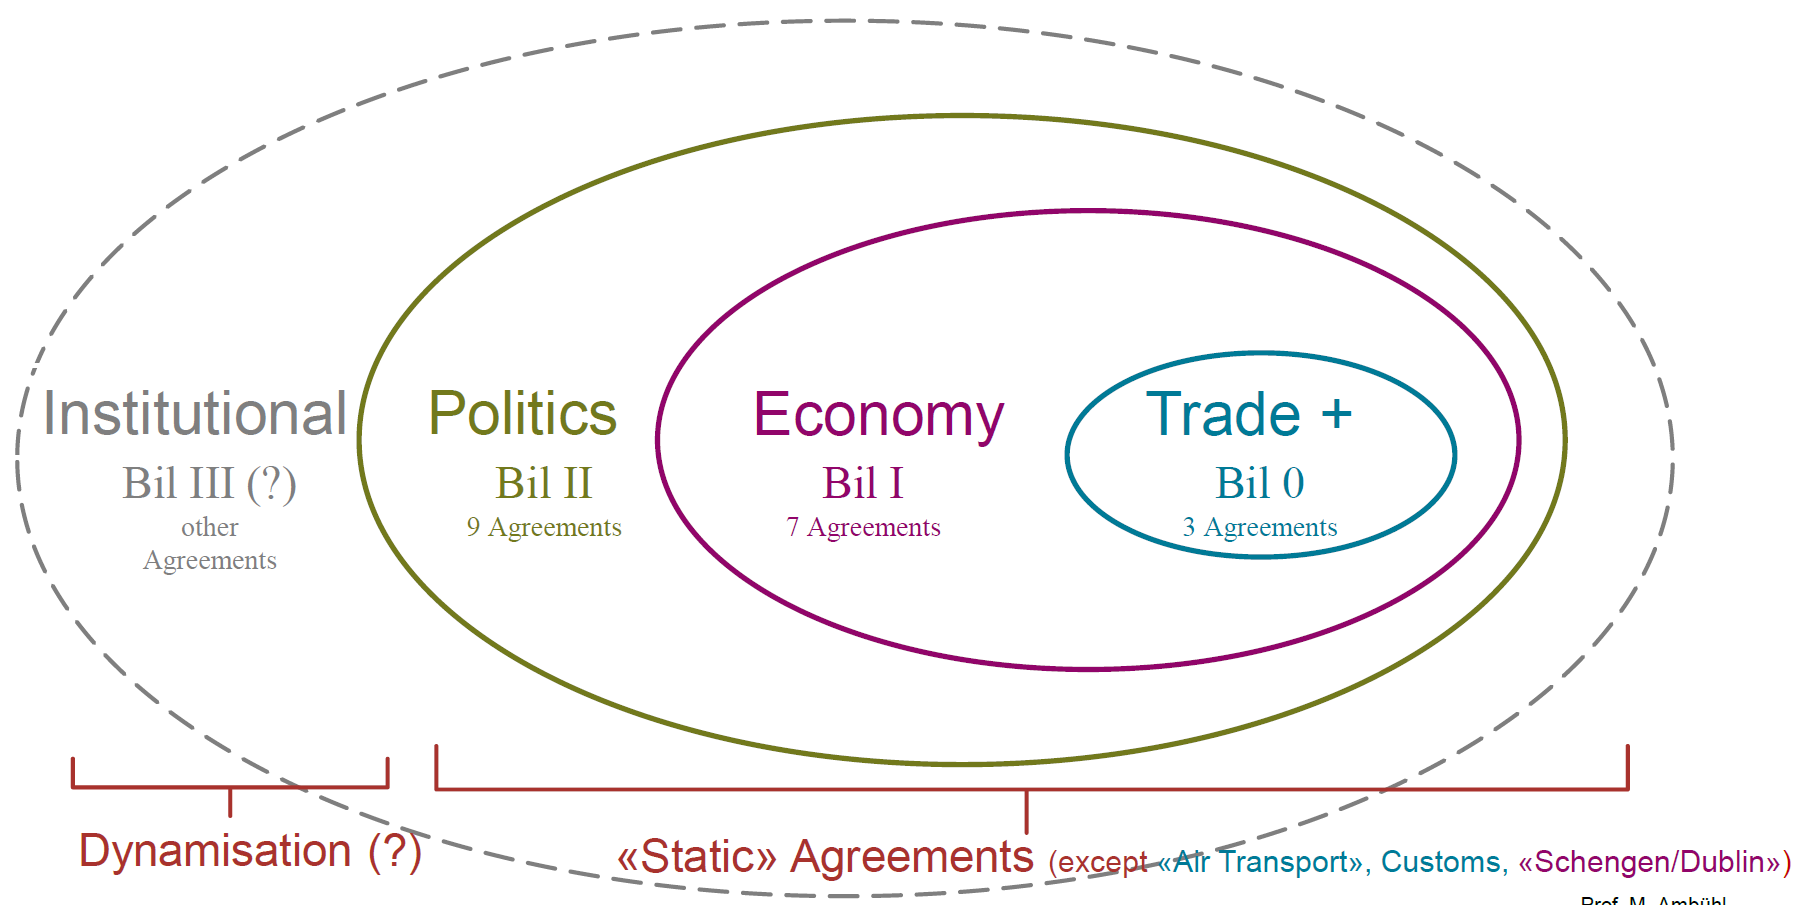
\includegraphics[width=0.8\textwidth]{Pictures/Swiss_Bilateral_Approach.png}
\end{figure}

\begin{enumerate}[]
    \item \underline{Bilateral $0$}: Free Trade Agreement, Insurance Agreement,
        custom's Agreement
    \item \underline{Bilateral \uproman{1}}: 7 sectoral agreements (linked
        together): Free movement of persons, Technical barriers to trade
        (MRA), Public procurement markets, Agriculture, Land transport,
        Air transport, Research.
    \item \underline{Bilateral \uproman{2}}: 9 sectoral agreements (not linked
        together): Schengen/Dublin, Taxation of savings, Combating fraud,
        Processed agriculture products, Environment, Statistics, MEDIA,
        Education, Pensions.
\end{enumerate}

\begin{figure}[h]
    \centering
    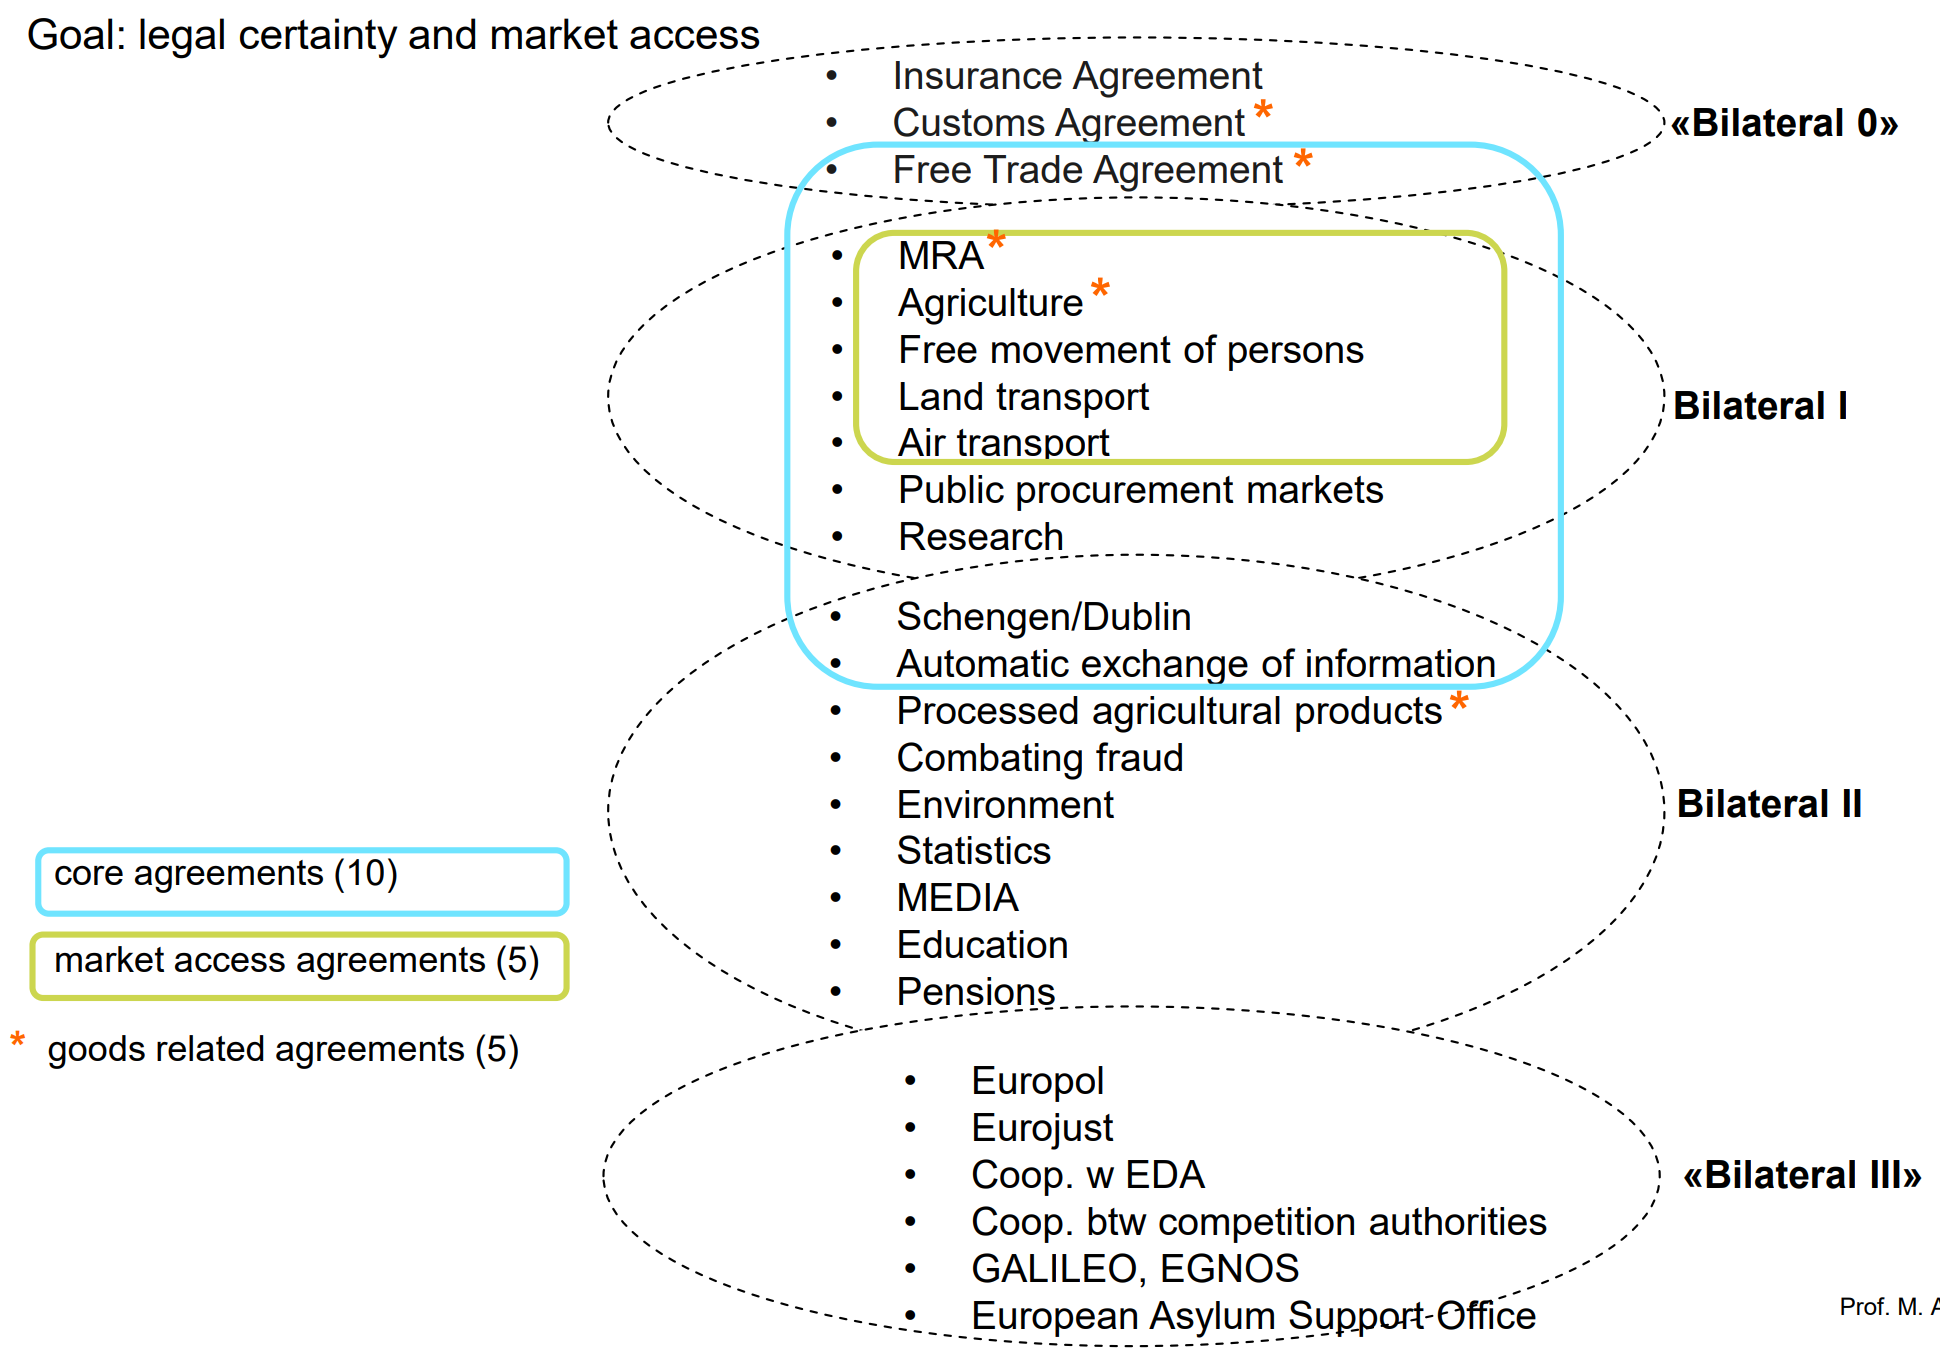
\includegraphics[width=0.7\textwidth]{Pictures/CH_EU_bilaterals.png}
\end{figure}

\paragraph{All in all}

\begin{itemize}
    \item Strong de facto integration
    \item Good relations through bilateral agreements
\end{itemize}

\paragraph{New challenges}

\begin{itemize}
    \item Institutional arrangements
    \item New market access agreements
\end{itemize}

\subsection{Cases}

\subsubsection{Land Transport Agreement CH-EU (1999)}

\paragraph{Background}

Bilateral \uproman{1}
\begin{itemize}
    \item Land transport
    \item Air transport
    \item Technical barriers to trade
    \item Public procurement
    \item Research
    \item Free movement of persons
    \item Agriculture
\end{itemize}

For the first two points declarations to negotiate existed, for the next
three where was a common interest and the last two were an EU-demand.

\subparagraph{Main challenges in the land-transport negotiations}

\begin{itemize}
    \item \underline{Internal}: Implementation of the Alpine Initiative Art. 84, Paragraph
        $2$ of the Swiss Constitution: "Transalpine goods traffic shall be
        transported from border to border by rail."
    \item \underline{External}: EU request:
        \begin{itemize}
            \item Abolishment of $28$t-limit
            \item No discrimination
        \end{itemize}
    \item $\Rightarrow$ Demanded: EU-compatible implementation of the
        Alpine Initiative.
\end{itemize}

\begin{figure}[h]
    \centering
    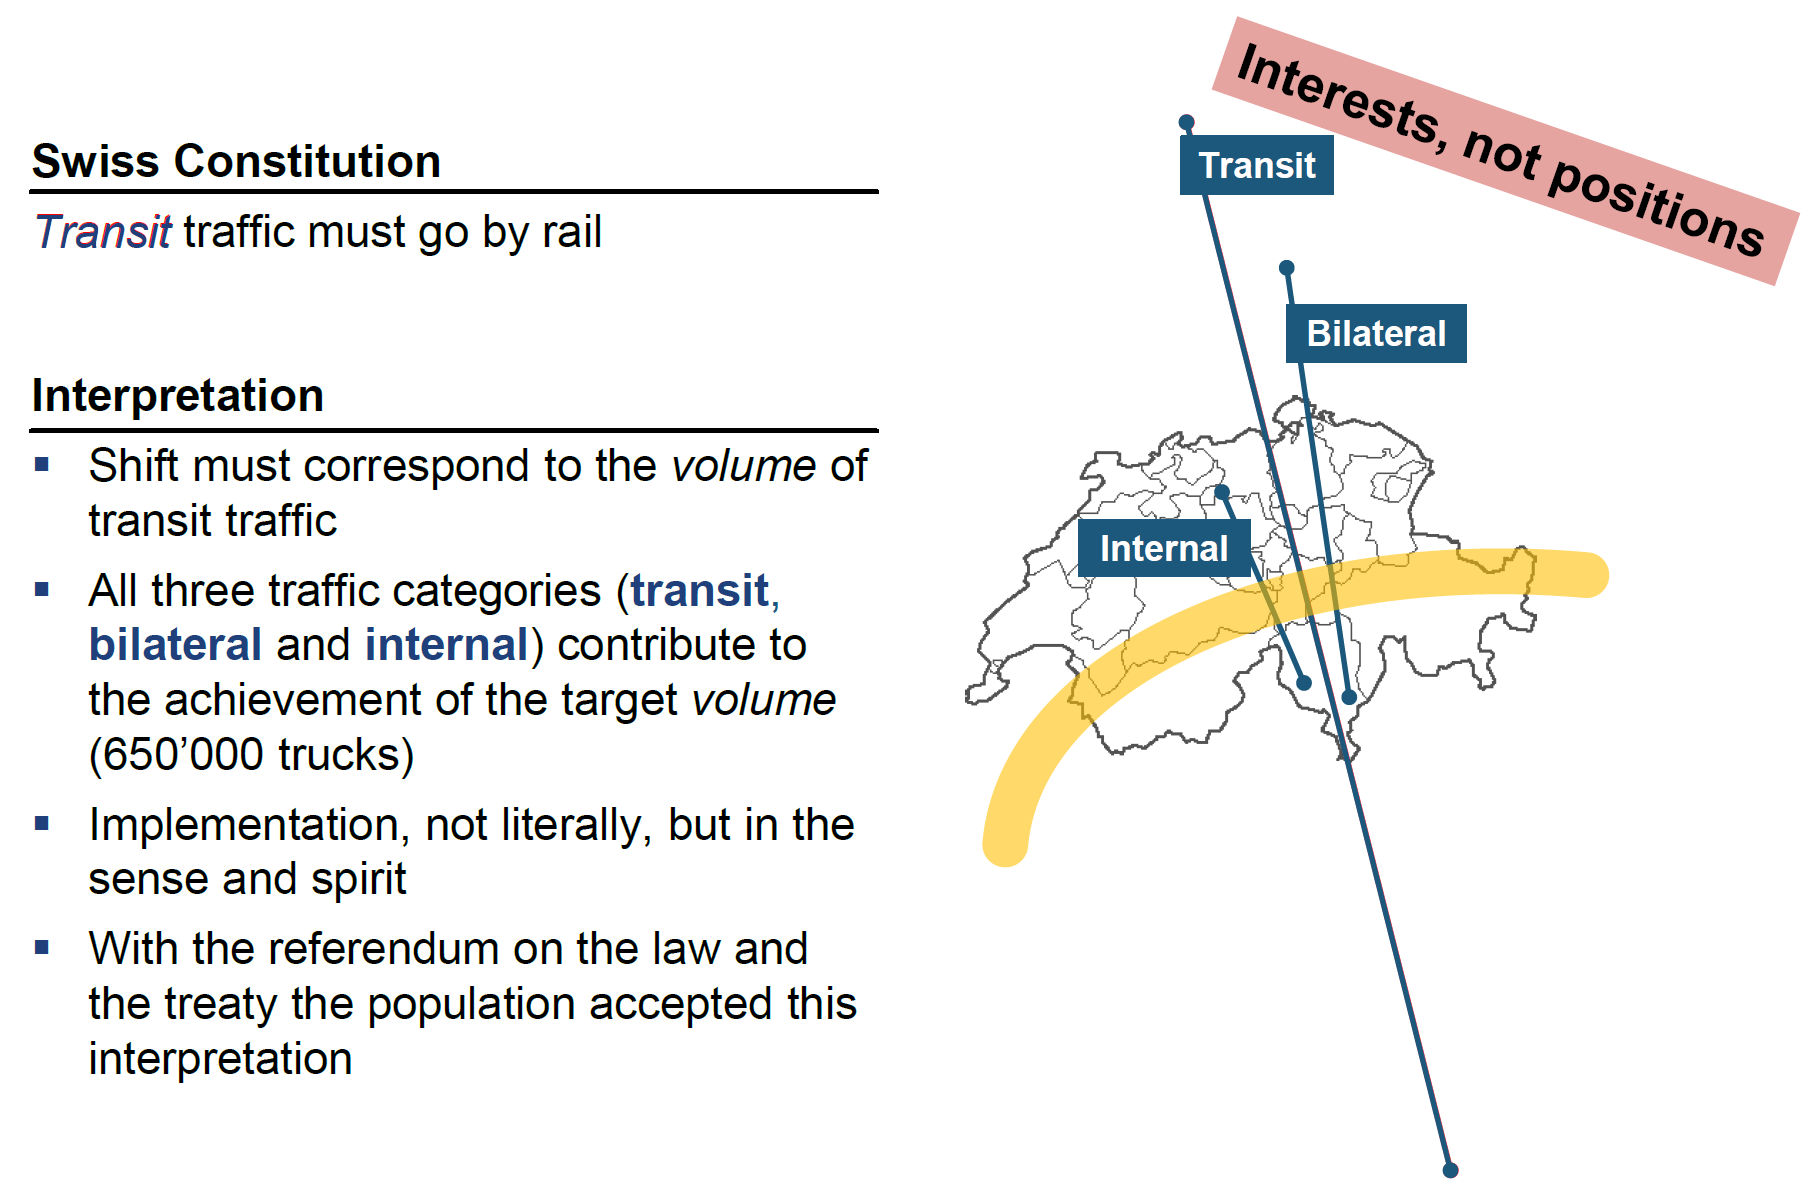
\includegraphics[width=0.7\textwidth]{Pictures/EU_CH_land_transport.png}
    \caption{Land Transport}
\end{figure}

\subparagraph{Negotiation challenges}

\begin{itemize}
    \item Complex political and technical question
    \item Discussion about ways and means to regulate truck traffic
    \item Consensus: regulation through pricing $\rightarrow$ tariffs
    \item Key-question: how to determine the amount?
\end{itemize}

\paragraph{Negotiation}

\subparagraph{Swiss proposal}
Environmental protection via market-based instruments (regulations by
means of pricing), rather than by command and control mechanisms
(steering by quotas):
\begin{itemize}
    \item Abolishment of the $28$t-Limit (zero quota for 40t trucks)
    \item Introduction of fees for trucks
\end{itemize}

\underline{Approach 1}: Tariffication of the weight limit

\begin{figure}[h]
    \centering
    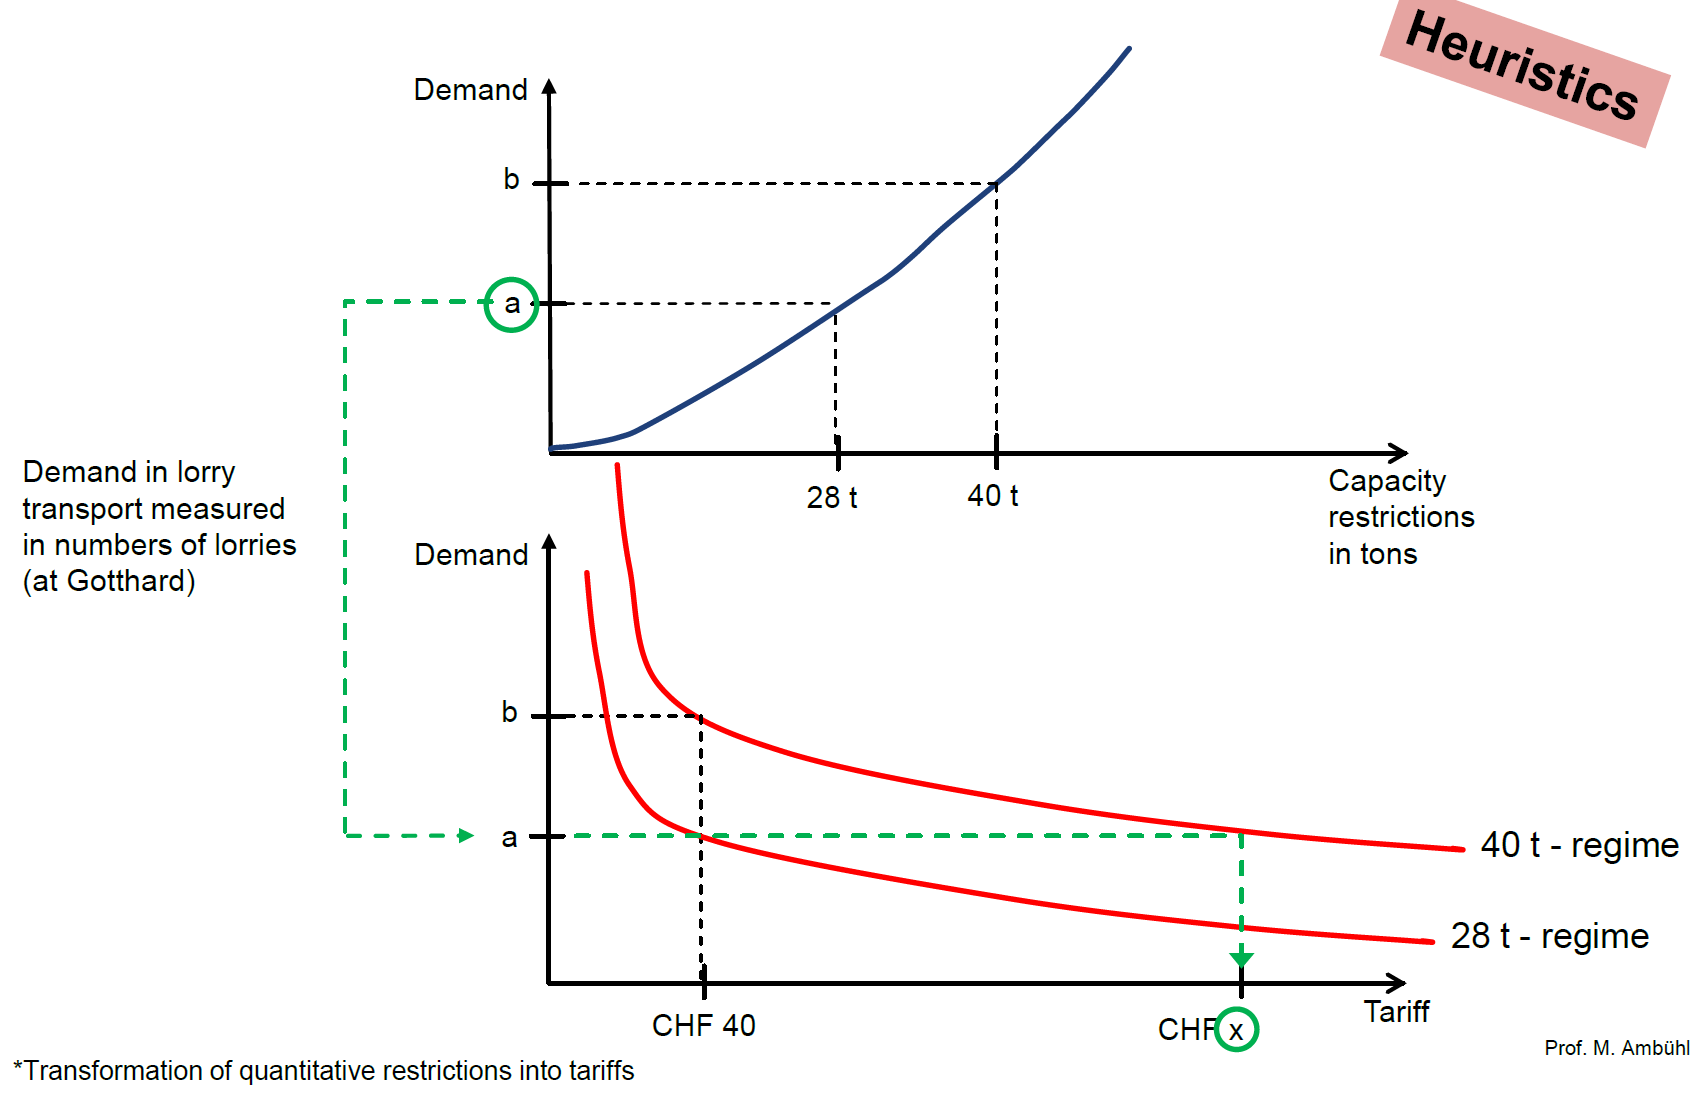
\includegraphics[width=0.8\textwidth]{Pictures/EU_CH_land_transport_approach_1.png}
\end{figure}

\underline{Approach 2}: Internalization of external costs
\begin{itemize}
    \item CH: CHF $560$ for $300$ km of a $40$ t lorry - internal and external costs
    \item Good concept, however EU did not like it for economic
        and political reasons.
\end{itemize}

\underline{Approach 3}: Pragmatic approach ("Negotiation Engineering")
\begin{itemize}
    \item Tariff split
    \item Weighted average
\end{itemize}


Main problem: different views on the amount: EU $200$ CHF $\leftrightarrow$
Switzerland $560$ CHF. Solution: Not $1$ tariff, but $3$ tariffs. Fixed
according to ecological criteria. New difficulty: Technological
development: Engines (cleaner trucks), Problem of Ökopunkte in Austria.
Solution: Weighted averages.

\begin{figure}[H]
    \centering
    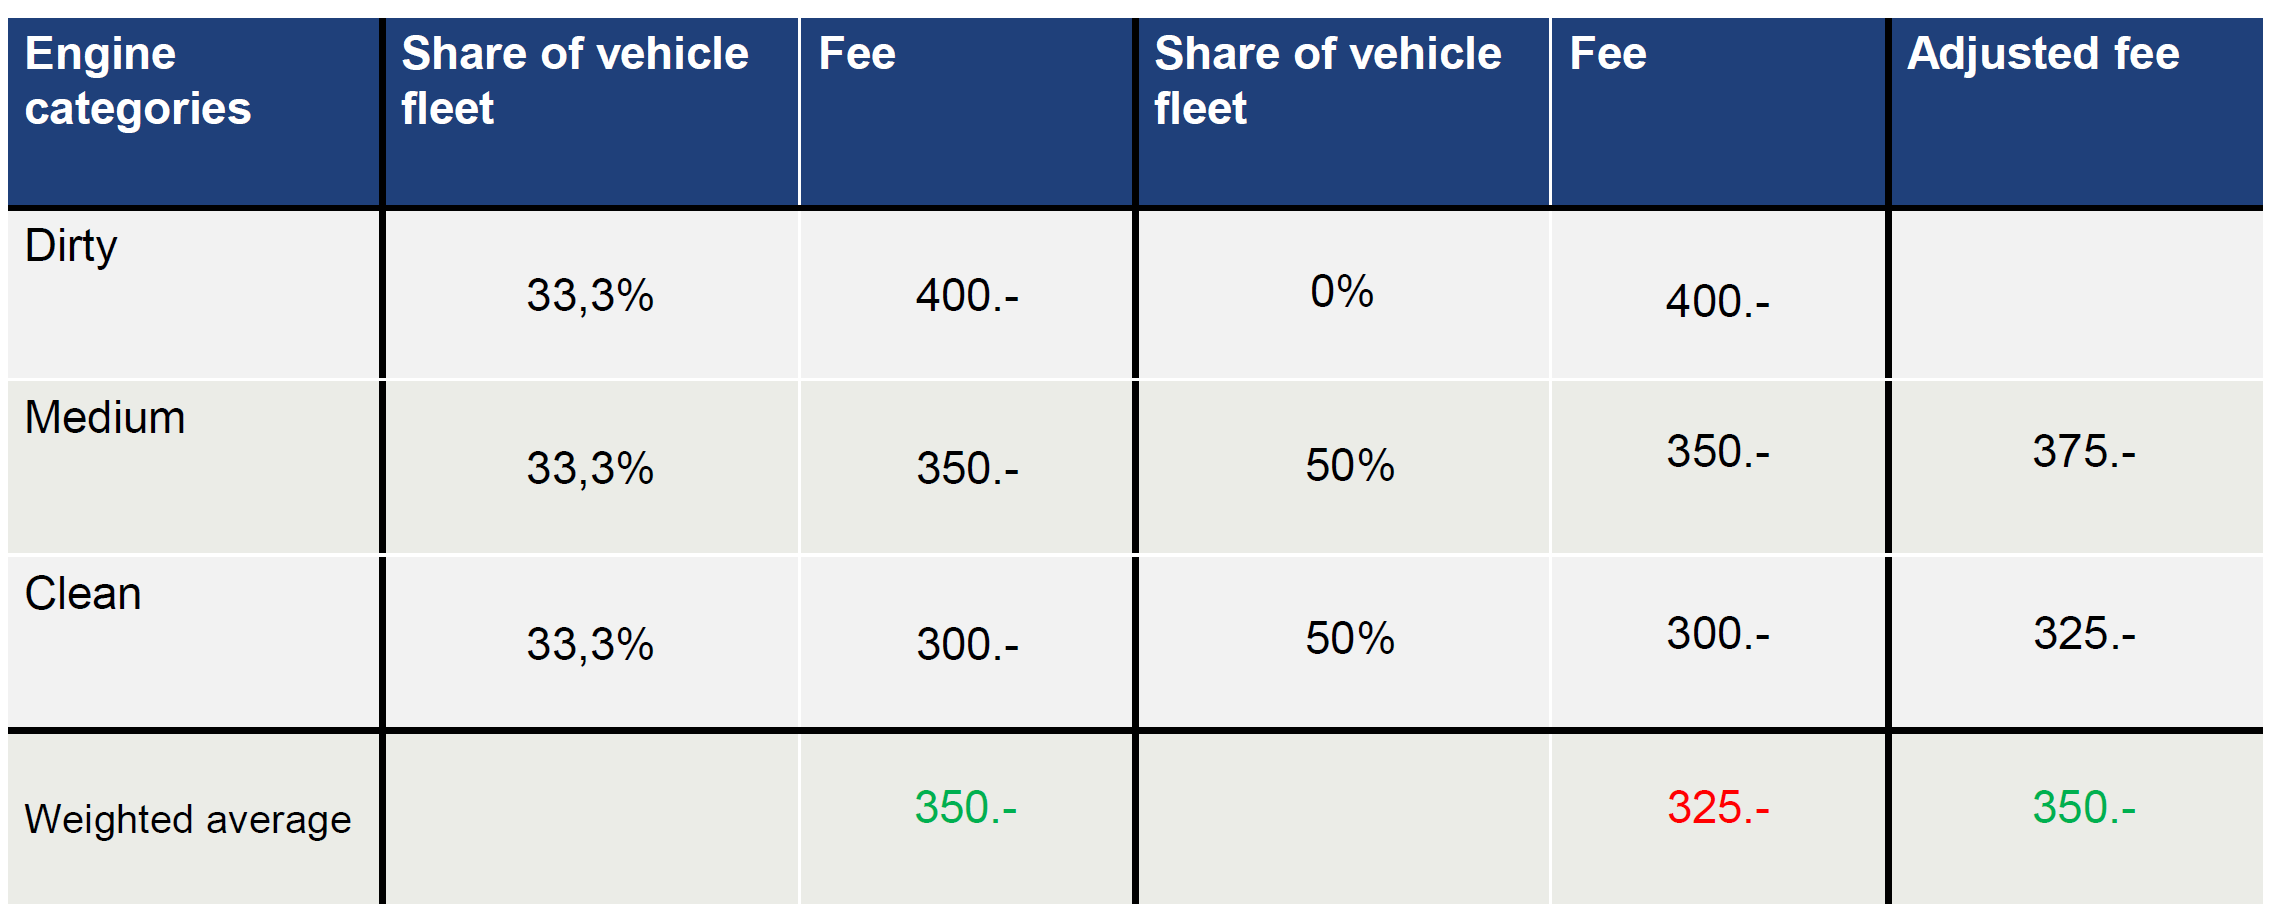
\includegraphics[width=0.8\textwidth]{Pictures/Land_transport_treaty.png}
\end{figure}

Calculation of fees for a given Weighted Average

\begin{itemize}
    \item $G$ - weighted average ($325.-$)
    \item $P$ - max tariff ($380.-$)
    \item $x,y,z$ - fees for lorries (dirty, medium, clean)
    \item $\alpha, \beta, \gamma$ - share of vehicle fleet of lorries (dirty, medium, clean)
    \item Optimization Problem:
        \begin{align*}
            &\max_{x,y,z} (x-z)
            \\
            &\alpha \cdot x + \beta \cdot y + \gamma \cdot z = G
            \\
            &x \leq P
            \\
            &0 \leq x - y \leq 0.15 \cdot G
            \\
            &0 \leq y - z \leq 0.15 \cdot G
            \\
            &x,y,z \geq 0
        \end{align*}
    \item Linear optimization problem $\rightarrow$ simple algorithm.
\end{itemize}

\paragraph{Comments}

\begin{itemize}
    \item Typical example of "negotiation engineering"
    \item Phases:
        \begin{enumerate}[1.]
            \item Negotiation of concept: Meccano / "Algebraic solution": $a,b,c,\dots,x,y,z$ etc.
            \item Try to solve as many "$a,b,c,\dots$" as possible
            \item Leave $2$ (max $3$) terms open, which can be decided in a final political
                / high level round
        \end{enumerate}
    \item Search for objective criteria is very useful
    \item Complicated calculation is sometimes helpful for political reasons:
        more difficult to criticize.
\end{itemize}


\subsubsection{Negotiation Menu (Bilateral \uproman{2})}

\paragraph{Background}

\begin{itemize}
    \item Four declarations in the Bilareral \uproman{1}:
        \begin{itemize}
            \item Three joint declarations ("Leftovers")
                \begin{itemize}
                    \item The Contracting Parties undertake a commence as soon
                        as possible negotiations on the general liberisation
                        of service provision on the basis of the acquis
                        communautaire.
                    \item The Comission of the European Communities and Switzerland
                        undertake to seek an appropriate solution to the problem of
                        the double taxation of the retirement pension of former
                        employees of institutions of the European Communities
                        resident in Switzerland.
                    \item The European Community and the Swiss Confederation declare
                        their intention to undertaking negotiations to conclude
                        agreements in areas of common interest such as the updating
                        of Protocol 2 to the 1972 Free Trade Agreement and Swiss
                        participation in certain Community training, youth, media,
                        statistical and environmental programmes. Preparatory work
                        for these negotiations should proceed rapidly once the current
                        bilateral negotiations have been concluded.
                \end{itemize}
            \item One unilateral declaration
                \begin{itemize}
                    \item Switzerland reaffirms its wish to reinforce cooperation
                        with the EU and its Member States in the area of migration
                        and asylum policy. To this end, Switzerland is willing to
                        participate in the EU system for coordinating asylum
                        applications, and it proposes that negotiations be
                        entered into for the conclusion of a convention
                        parallel to the Dublin Convention (Convention determining
                        the State Responsible for examining applications for
                        Asylum lodged in one of the Member States of the
                        European Communities, signed in Dublin on 15 June 1990).
                \end{itemize}
        \end{itemize}
    \item Demand of the EU regarding:
        \begin{itemize}
            \item Savings taxation
            \item Fight against Fraud
        \end{itemize}
\end{itemize}
$\rightarrow$ 10 subjects of Bilateral \uproman{2} negotiations. Later
reduced to 9, Liberization of services was dropped.


\begin{itemize}
    \item CH and EU in the beginning of the "Bilateral \uproman{2}"-negotiation
        did not agree on the "menu" (i.e. the issue to be negotiated)
        \begin{itemize}
            \item CH wanted all 10 issues mentioned earlier in one or another form
            \item EU wanted only 6 issues in a first phase and, depending on the
                outcome in the fraude-dossier, eventually a second phase for the
                4 issues:
                \begin{itemize}
                    \item Schengen/Dublin
                    \item Services
                    \item Education/Youth
                    \item Media
                \end{itemize}
        \end{itemize}
    \item CH insisted on the parallelism in the negotiations (we learnt our
        lessons of Bilateral \uproman{1})
    \item EU did not want a parallelism
\end{itemize}

\paragraph{Negotiation}

\begin{figure}[H]
    \centering
    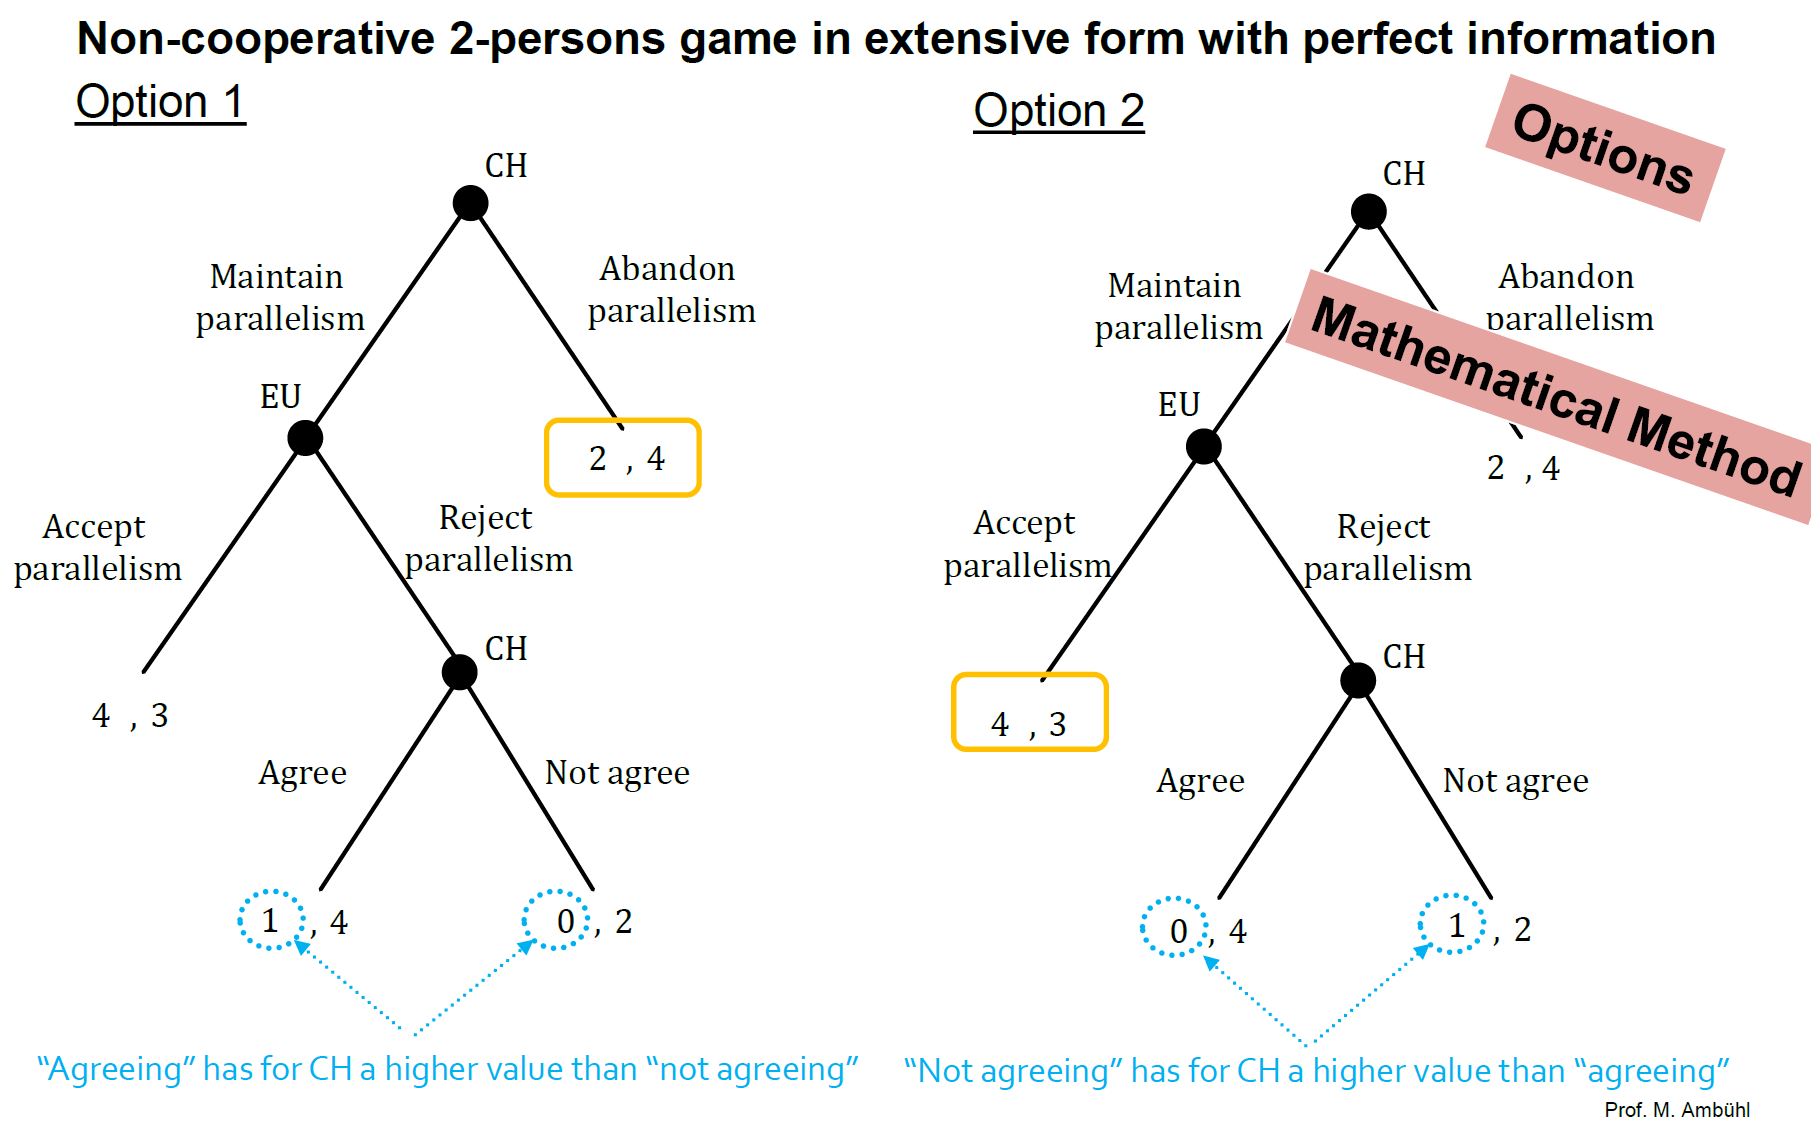
\includegraphics[width=0.7\textwidth]{Pictures/Bilateral_2_negotiation.png}
    \caption{Negotiation}
\end{figure}

\paragraph{Results}

\begin{itemize}
    \item Switzerland decided on option 2 (insisting on parallelism)
    \item EU finally agreed, on 17.06.2002, to start the negotiation on all 10 issues
    \item Berne/Brussels started with the negotiation on 18.6.2002
    \item Initialed: 25.06.2004
    \item Signed: 26.10.2004
    \item Vote: 5.6.2005
    \item In force: 2005 (different dates for agreements)
\end{itemize}

\paragraph{Comments}
\begin{itemize}
    \item Rare case, known to me ($\sim$20 cases), where a government took
        a decision (March 2002) based on a game theoretical analysis
    \item It was to Switzerland's advantage and allowed to include Schengen
        negotiation
    \item Game theoretical sensitivity analysis helped to convince the own
        decision makers and to make the right decision
\end{itemize}


\subsubsection{Schengen Association Agreement}

\paragraph{Background}

\begin{itemize}
    \item Schengen and Dublin are integral parts of the EU-Acquis
        (The EU Acquis are the accumulated legislation, legal acts, and
        court decisions which constiturte the body of EU law.)
    \item Third country has to take over the whole Acquis; in case of
        development of the Acquis, the third party has to take over the new
        Acquis.
    \item The third party has no decision-making rights, only decision-shaping rights
    \item In the case where the third country does not take over the new Acquis and
        the parties do not find a pragmatic solution, then "Guillotine" applies.
\end{itemize}

\paragraph{Negotiation}

\begin{itemize}
    \item CH accepted the fact that Schengen/Dublin is an integration/dynamic agreement
    \item However, CH wanted a special exeption regarding the judical assistance
        concerning Art. 51 of the "Convention Implementing the Schengen
        Agreement" (CISA/SDÜ) 1990
\end{itemize}

\subparagraph{Summary Article 51}

a)
Act is punished with more than 6 months of imprisonment in both contracting
parties, A and B. Or: Act is pinishe with more then 6 months of imprisonment
in A, and is prosecuted by administrative authorities in B (with the
possibility to appeal to a court which has jurisdiction in criminal matters)

\paragraph{Results}

\begin{figure}[H]
    \centering
    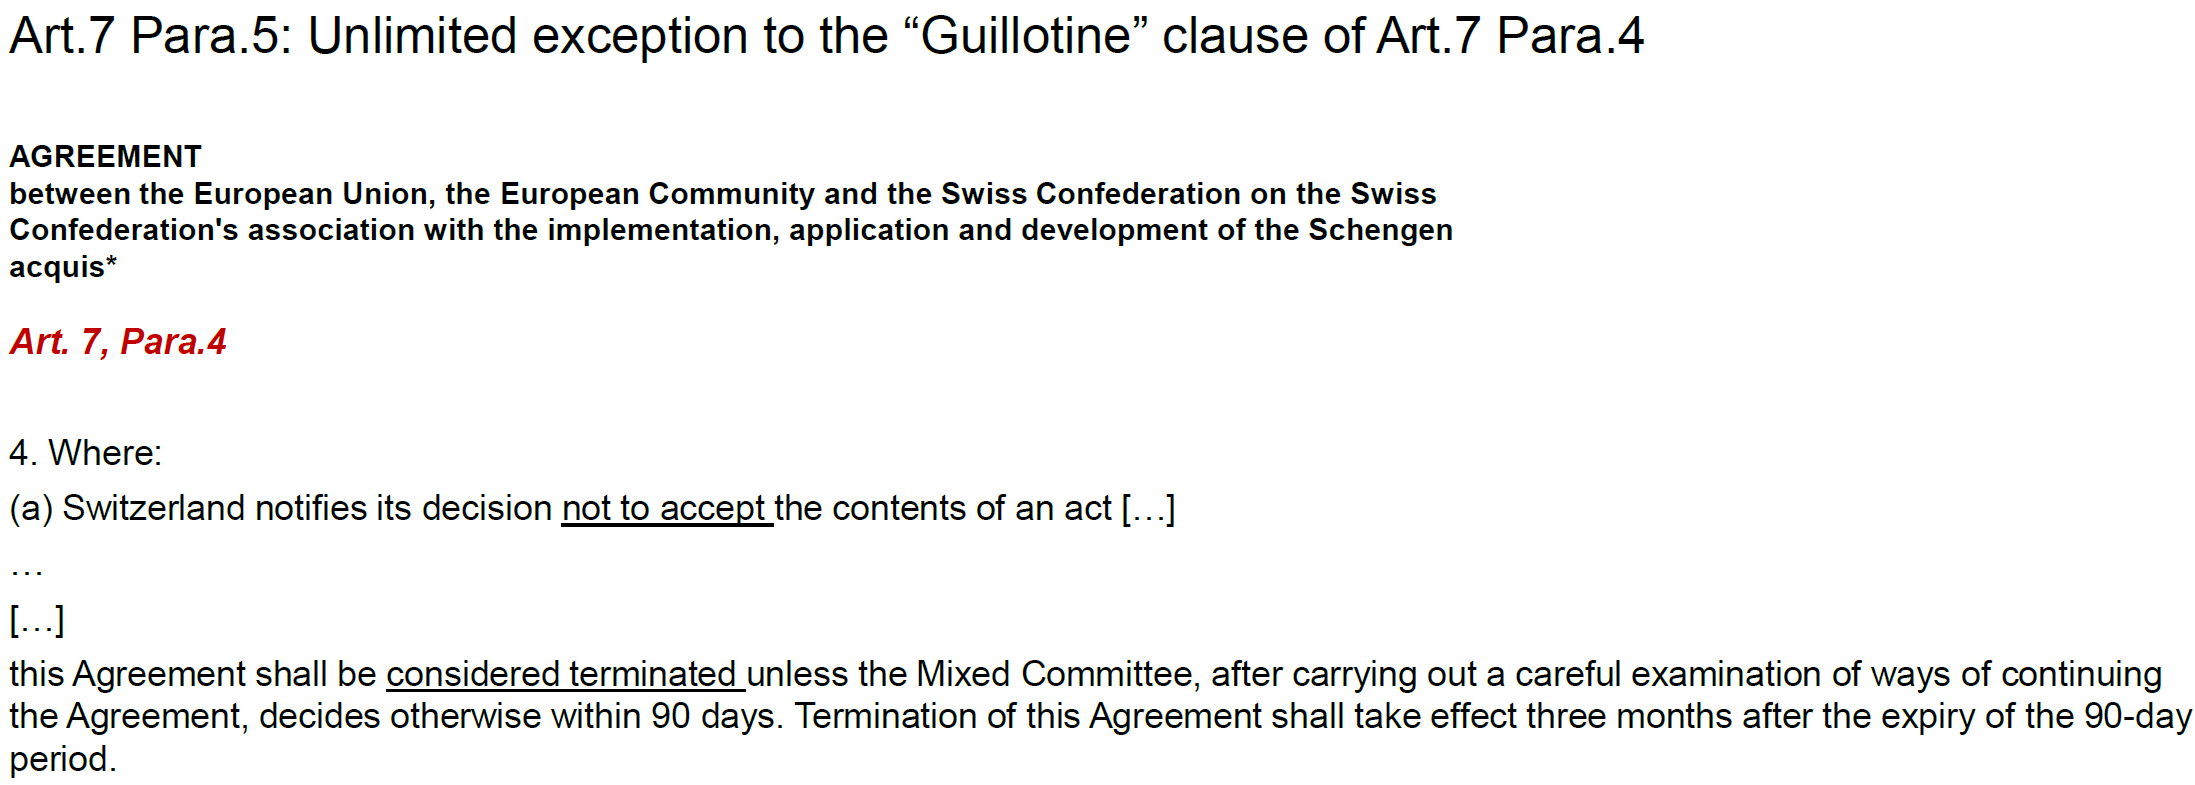
\includegraphics[width=0.9\textwidth]{Pictures/Schengen_result_1.png}
    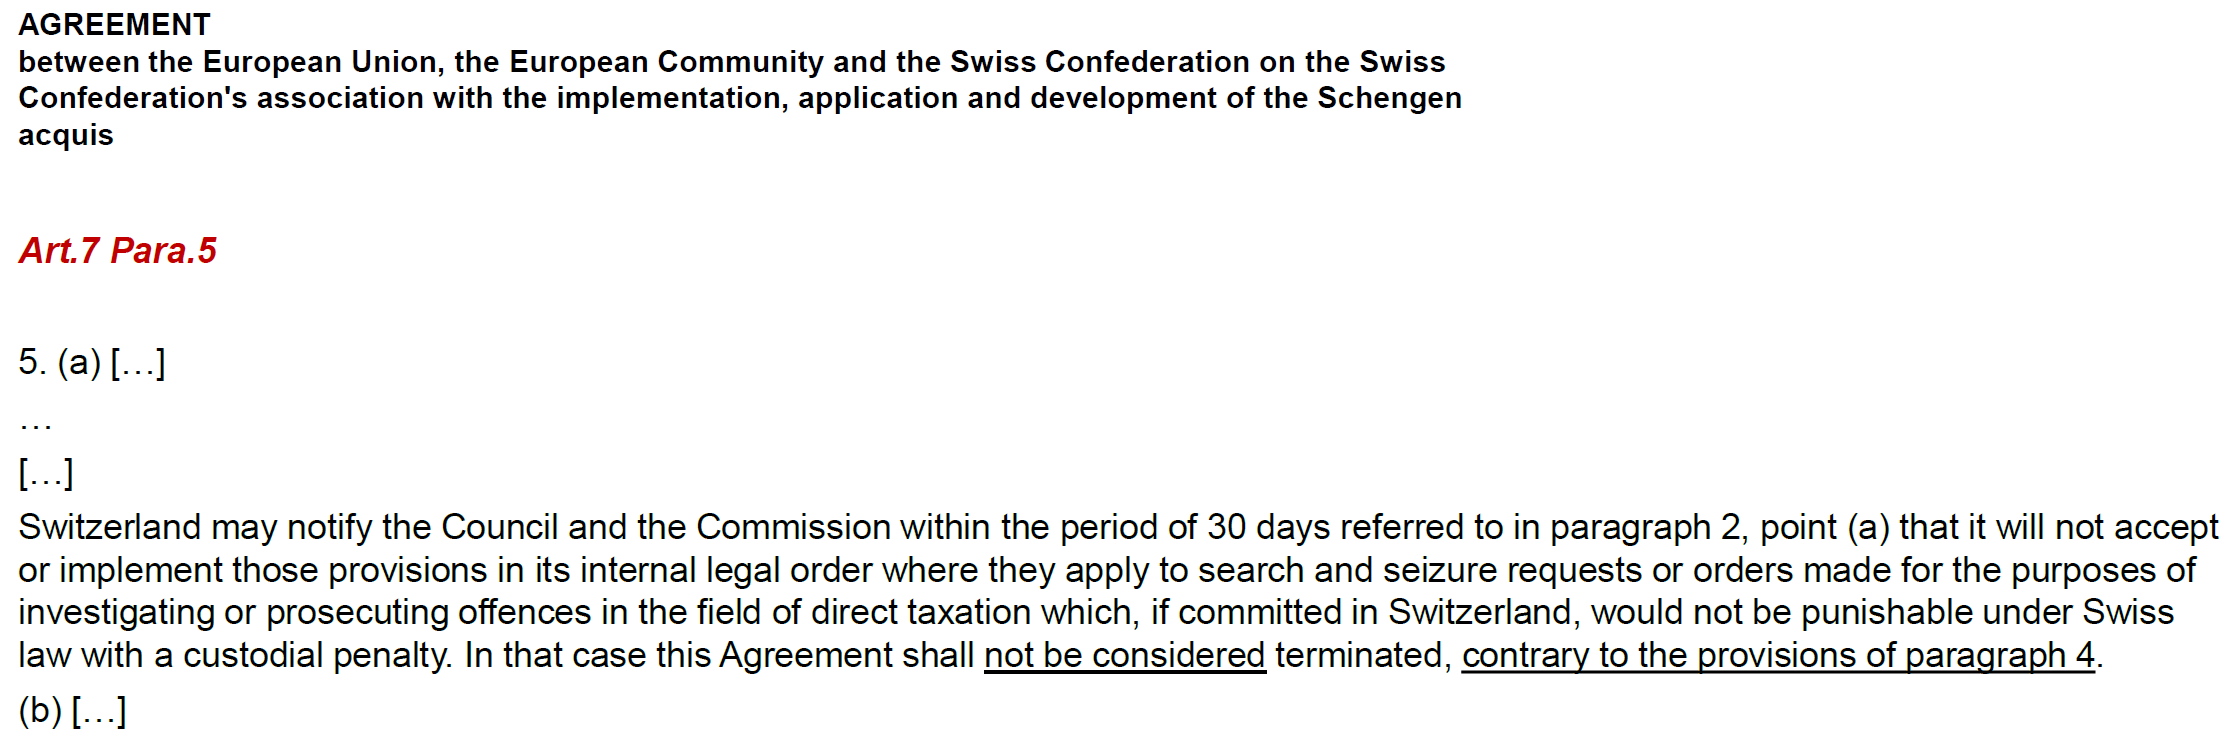
\includegraphics[width=0.9\textwidth]{Pictures/Schengen_result_2.png}
    \caption{Results}
\end{figure}


\paragraph{Comments}

\begin{itemize}
    \item It is important to have reasonable (counter-) demands
        \begin{itemize}
            \item Co-decision would not have been one
            \item Exception of Art. 51 was a border line case
        \end{itemize}
    \item Thanks to the strong demand of the EU in savings taxation and
        to the tight line between the subjects made by CH
        $\rightarrow$ CH succeeded
\end{itemize}


\subsubsection{Institutional Agreement (Current Case)}

\paragraph{Background}

\begin{itemize}
    \item Most bilateral agreements between EU and Switzerland are of static
        nature; i.e. if the EU-Acquis changes, the bilateral agreements do not
        change dynamically.
        \begin{itemize}
            \item \underline{Advantages}: Switzerland knows what "the rules"
                are and may reject changes.
            \item \underline{Disadvantages}: EU can withhold changes Switzerland
                would like to accept and use this as a bargaining chip in order
                to achieve its goals in other issues.
        \end{itemize}
    \item EU wants to embed existing bilateral market access-agreements with
        Switzerland within an institutional framework in order to change the
        static nature to a dynamic nature and in order to implement a dispute
        settlement process.
    \item For the time being, negotiations for corresponding draft agreement
        (InstA) were "concluded" (EU view) / "suspended" (CH view) in November
        2018.
    \item The Federal Council decided to launch a broad domestic consultation.
    \item In June 2019, the Federal Council decided to ask for 3 clarifications
        of the text.
    \item After these clarifications, the Federal Council is faced with the
        decision whether to sign the InstA or not.
\end{itemize}

\paragraph{Negotiations}

\begin{itemize}
    \item EU signaled its interest in changing the bilateral agreement from
        a static nature to a dynamic nature already over 12 years ago.
    \item For Switzerland the static nature has certain advantages, nevertheless
        dynamization remains a major concession.
    \item EU: most important international partner and with more bargaining power.
    \item Switzerland could accept dynamization, if safeguards are established:
        exceptions for areas of vital interest and a truly independent dispute
        settlement process.
    \item Hence the Federal Council decided to pursue such negotiations by
        defining a mandate in 2013.
    \item In November 2018, the negotiations came to a tentative end in the
        form of a draft agreement/InstA. Switzerland did neither reject nor
        accept $\rightarrow$ domestic consultation.
    \item CH did not reject it. Reason: EU imposed time limit for the
        recognition of equivalence of the stock market.
\end{itemize}

\paragraph{Result}

We focus on 5 issues:
\begin{enumerate}
    \item Achievement to negotiate an institutional framework
    \item Horizontal joint committee might contribute to foster the
        political exchange between Switzerland and the EU
    \item The dispute settlement process envisages that in case of disputes for
        which the joint committe cannot find a solution, either party may request
        to refer the dispute to an arbitration panel. If resolving the dispute
        requires clarification of a question concerning the interpretation or
        application of EU law, the arbitration panel refers the matter to the
        CJEU. The arbitration panel then resolves the matter based on the CJEU's
        interpretation. As the bilateral agreements are by definition mostly
        related to EU law, the CJEU's ruling might be decisive in most cases.
    \item The so-called "guillotine clause" is further extended within the InstA.
        (Reminder: the existing guillotine clause connects the 7 agreements of the
        Bilateral \uproman{1} package.) Should the InstA be terminated, not only
        will the InstA cease to be in force but also all future market access
        agreements. Should the parties not be able to agree otherwise within 3
        months, the 5 agreements of the Bil \uproman{1} package, which are affected
        by the InstA will no longer be in force. Due to the existing guillotine
        clause, the same applies for the remaining 2 agreements of the Bil \uproman{1}
        package. Furthermore, the same most likely also applies for Schengen-Dublin
        as this agreement in only possible within a "free movement of person's area".
        Summarizing: The "default value" is to terminate the mentioned agreements
        (as opposed to another "default value", which envisages not to terminate
        the agreements, except if one party actively decides to do so.)
    \item In certain areas, which are vital for Switzerland, the negotiations
        were able to achieve an explicit exception from the dynamization (e.g.
        land transport) However, other vital areas (e.g. accompanying measures,
        the state subsidies, Citizen's Rights Directive) were not fully excluded.
\end{enumerate}

\paragraph{Comment}

Assessment:
\begin{itemize}
    \item Generally, it is good for Switzerland to have an institutional
        agreement in order to consolidate the bilateral path.
    \item Horizontal joint commitee potentially facilitates political dialog.
    \item The dispute settlement process as desiged in the InstA might not be
        unproblematic: CJEU is the court of one party. In international law it
        is rather unusual that a party subjects itself to the jurisdiction of
        the other party (even if this court might be a well-reputed one).
    \item The extension fo the guillotine clause is no longer politically
        legitimate in a dynamic framework, which foresees the introduction
        of "rebalancing measures".
    \item Based on domestic consultation process, the protection of salaries
        is not sufficient; the Union Citizens' Rights Directive is considered,
        by certain circles, to be problematic.
\end{itemize}

Our propositions:
\begin{itemize}
    \item Exceptions of dynamization in vital areas
    \item Simplified dispute settlement process (inspired by existing CH-EU
        custom's agreement of 2009)
    \item No extension of guillotine clause but elimination or relativization.
\end{itemize}

\vspace{1\baselineskip}

\fat{Ad dispute settlement process}:

\begin{figure}[h]
    \centering
    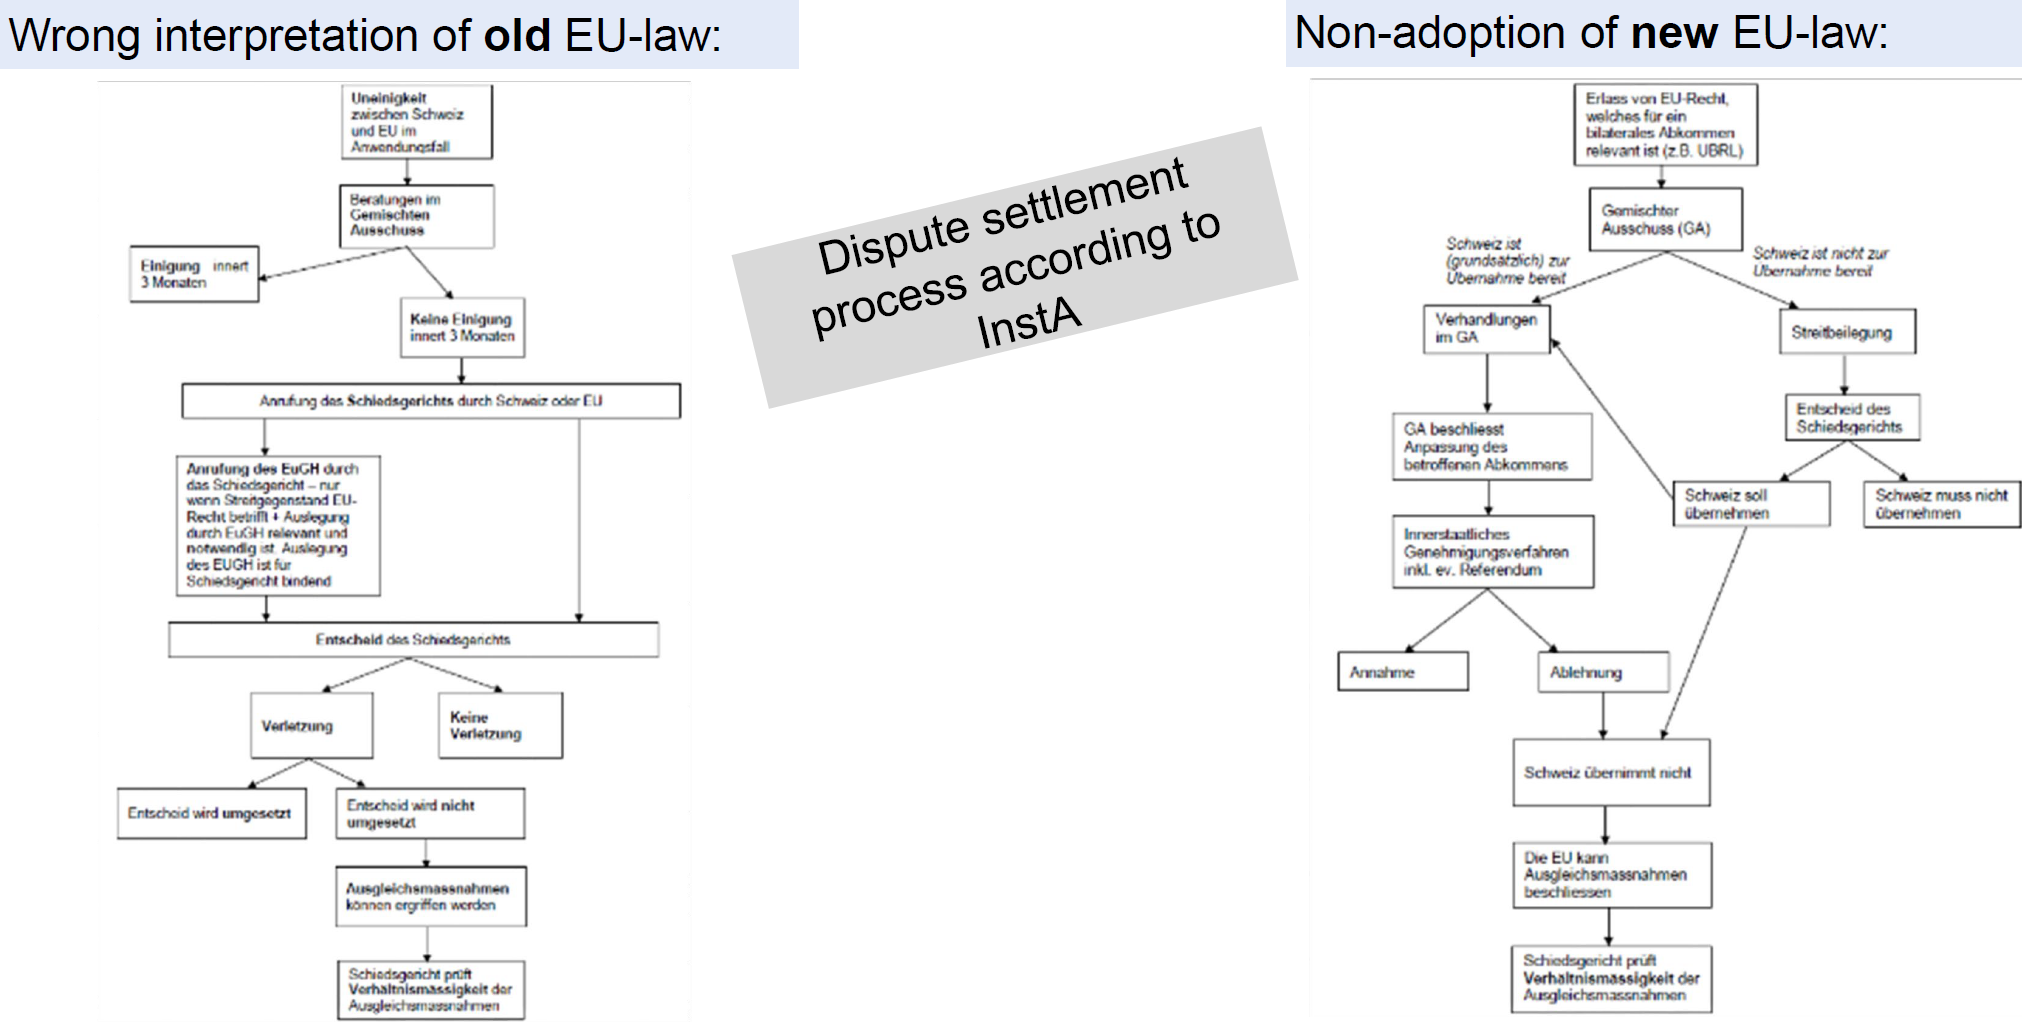
\includegraphics[width=\textwidth]{Pictures/dispute.png}

    \vspace{1\baselineskip}

    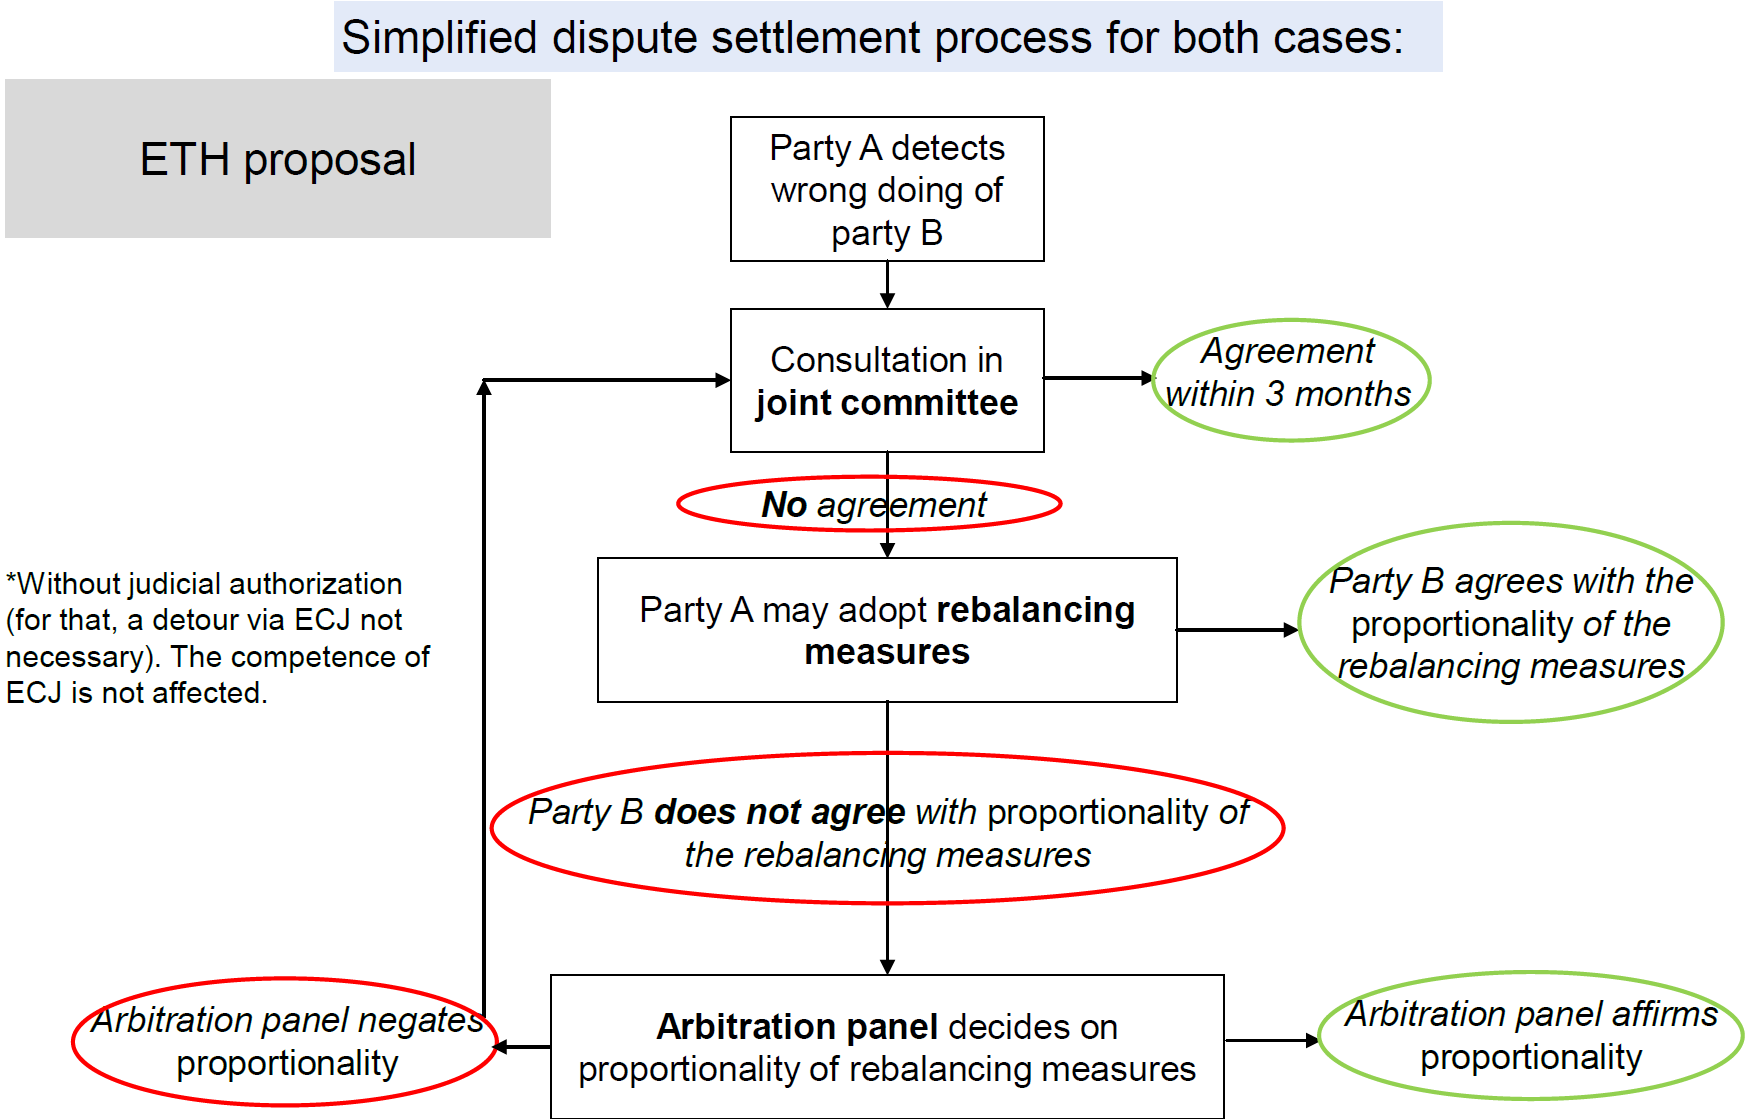
\includegraphics[width=0.8\textwidth]{Pictures/simplified_dispute.png}
\end{figure}


\paragraph{Summary of our assessment}
\begin{itemize}
    \item A framework agreement is desirable.
    \item The present draft agreement has deficiencies, which narrow the domestic
        political acceptance.
    \item According to us, if the Swiss Government would conclude that the
        probability of a rejection in a Swiss referendum is higher than the
        acceptance, then it should not sign the draft agreement. A no vote by
        the Swiss population does more damage to our bilateral relations than
        a suspension of the negotiation on the level of the negotiators.
    \item In such a case, both sides should concentrate on an Interim Agreement
        with concrete positive measures.
\end{itemize}

\hrule

\paragraph{InstA follow up (2021)}

\begin{itemize}
    \item The meeting between Swiss President Guy Parmelin and Com President
        von der Leyen on 23.4.21 in Brussels has brought clarity.
    \item There exists some substantial differences regarding salery protection,
        right of citizens of the Union, (and to a lesser extend, susidies)
    \item What to do? 3 Options
        \begin{itemize}
            \item Continue the negotiations and potentially sign the agreement
            \item Stop the negotiations without Plan B
            \item Stop the negotiations with a Plan B
        \end{itemize}
    \item Concerning the Plan B:
        \begin{itemize}
            \item (i) Unilateral offer after stopping the negotiations
            \item (ii) bilateral agreement, may be an "InstA light"
                \begin{itemize}
                    \item dynamization, with 2 "opt outs" (salary protection, UBRL)
                    \item simplified dispute settlement acc to our ETH model
                    \item cohesion payment's increase
                    \item new agreements: electicity, research, health
                    \item review clause
                \end{itemize}
        \end{itemize}
\end{itemize}


\hrule


\subsubsection{Refugee Distribution}

\paragraph{Background}

\begin{itemize}
    \item EU is currently dealing with the largest refugee crisis since WW2;
        Germany alone has received 1.1 Mio refugees in 2015.
    \item EU and EFTA have a common asylum policy governed by the Dublin
        \uproman{3} Regulation (except for Denmark); this regulation essentially
        obliges refugees to apply for asylum in the EU/EFTA state in which they
        first enter.
    \item $\Rightarrow$ Stong asylum pressure for several Southern European
        states (=entry points for most refugee routes)
\end{itemize}

\paragraph{Negotiation}

Stong opposing position within the EU/EFTA:

\begin{figure}[h]
    \centering
    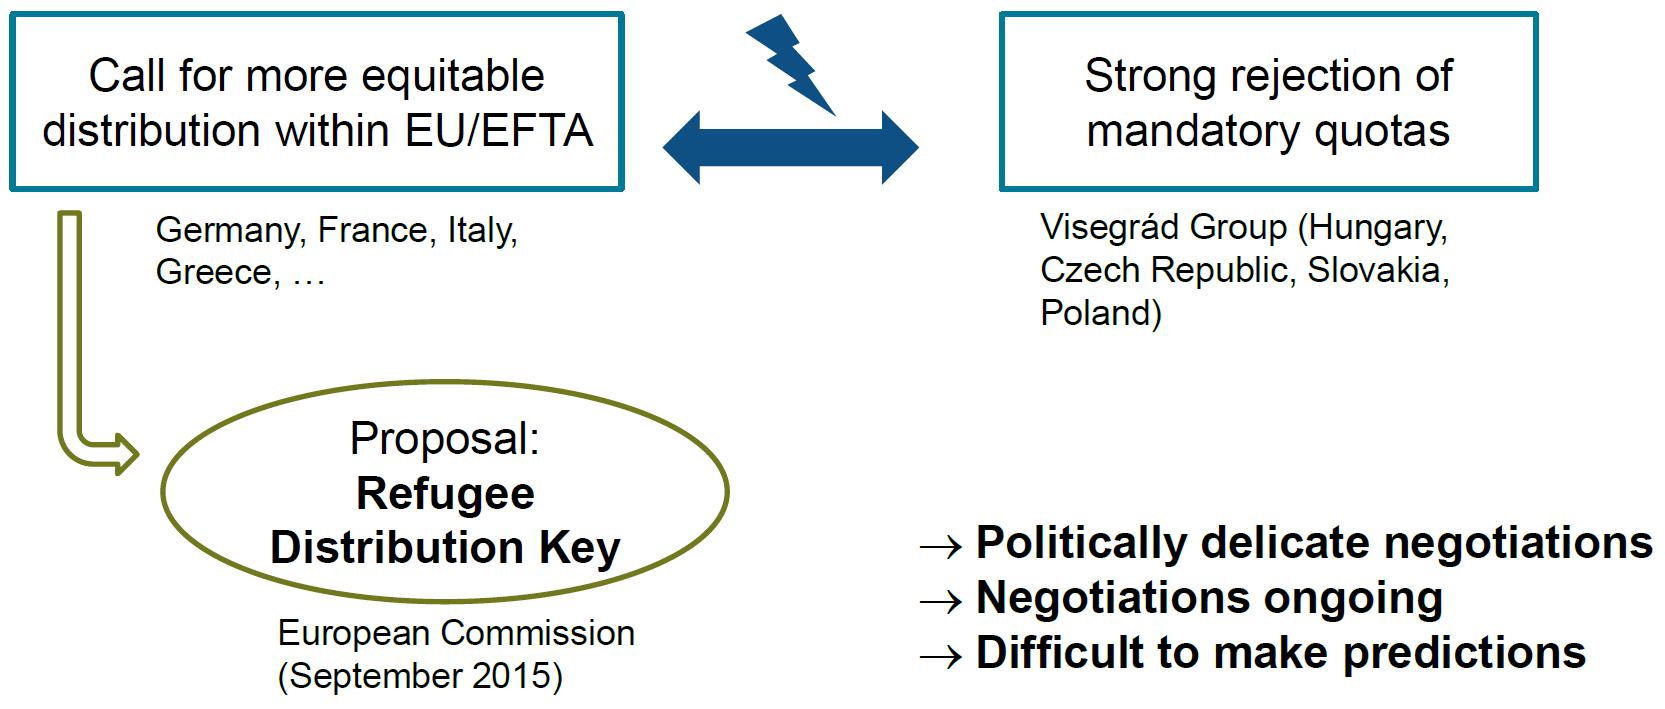
\includegraphics[width=0.6\textwidth]{Pictures/refugees.png}
\end{figure}

\paragraph{Result}

Regulations made with mathematical methods.
The distribution key formula determines, for each state, the fraction of
all asylum applications that it has to deal with. It is based on the following
four influencing factors:
\begin{enumerate}
    \item GDP
    \item Population Size
    \item Corrective factor: Average number of asylum applications per one
        million inhapitants over the preceeding five years
    \item Corrective factor: Unemployment
\end{enumerate}

Press Release European Commission (September 2015):
"Corrective factors for the average numbers of asylum applications and unemployment
rate are applied inversely, meaning that high existing asylum application numbers
and a high unemployment rate would result in fewer individuals being relocated
to a member state".

\vspace{1\baselineskip}

The conclusion is incorrect. The formula was wrong.

\paragraph{Fact (undesired property)}
\begin{itemize}
    \item Some states with comparably high unemployment and high number of
        past asylum applications per capita receive a higher quota than if the
        two corrective factors were not taken into account.
    \item Conversly, states with comparably low unemployment and few past asylum
        applications per capita may actually benefit from a diminished asylum
        burden due to the corrective factors.
    \item Key reason for the undesired properties: Population size and GDP are
        treated in the same way as unemployment and past asylum applications.
\end{itemize}

\paragraph{Comment}

\begin{itemize}
    \item The European Commission's approach is a classical example for
        negotiation engineering
    \item Their formula however suffers from an international inconsistency.
        This can be seen by a heuristic argument and data analysis.
    \item Keep formulas simple and transparent and apply sanity checks to
        ensure their consistency (engineering mindset)
\end{itemize}

A detailed account of the described inconsistency as well as proposal for an
alternative distribution key can be found in (to appear in "European Union
Politics").


\subsection{Conclusions}

\begin{enumerate}
    \item Negotiations with EU are bilateral and multilateral and most often
        complex:
        \begin{itemize}
            \item Several players
            \item Smallest commmon denominator
            \item Concept of bilateral negotiations is basically against EU
                EU logic. Four categories of countries:
                \begin{itemize}
                    \item EU-Member States (w-w/o Schengen; w-w/o Euro)
                    \item EEA (EU + Norway + Iceland + Lichtenstein)
                    \item Candidate countries
                    \item Third countries
                    \item $\text{[Brexit (new category?)]}$
                \end{itemize}
        \end{itemize}
    \item Co-decision rights
        \begin{itemize}
            \item "EU-ins":
                \begin{itemize}
                    \item Have more to say
                    \item But have to follow rules and can be outvoted
                \end{itemize}
        \end{itemize}
\end{enumerate}

\pagebreak

\hrule

\subsubsection{Box: EU-Institutions}

\begin{itemize}
    \item Complicated basic structure: mixture between Confederation and Federation.
    \item Decision making in small groups, dominance of big powers.
    \item Evolution of the percentage of votes for DE, FR, IT:
        \begin{itemize}
            \item $23.5\%$ (EEC6)
            \item $15.9\%$ (EC10)
            \item $11.5\%$ (EU15)
            \item $8.4\%$ (EU27)
            \item $8.2\%$ (EU28)
        \end{itemize}
    \item Is there a Voting Paradox? Losing voting weight but gaining incluence(?)
    \item Pro memoria: Percentage of votes system has been abandoned: Art. 16(4)
    of the Lisbon Treaty (TEU). See Brainteaser 4!
\end{itemize}

\hrule

\vspace{1\baselineskip}

\begin{enumerate}
    \setcounter{enumi}{1}
    \item Co-decision rights
        \begin{itemize}
            \item "EU-outs" hold "good cards" only if they:
                \begin{itemize}
                    \item have a nuisance value (Störpotential) / leverage
                    \item make a positive contribution to the good functioning
                    \item do not intend to go against EU essentials
                \end{itemize}
        \end{itemize}
    \item Best strategy for a smaller player
        \begin{itemize}
            \item Coherent concept / proposal and no contradictions
            \item No changes in argumentation
            \item Make reasonable counter-demand
            \item Don't say "No", say "Yes, but\dots"
        \end{itemize}
    \item Way forward in negotiations
        \begin{itemize}
            \item Identify interests of both sides
            \item Develop concepts based on:
                \begin{itemize}
                    \item Objectives, principles, measures, special modalities,
                        safeguard clauses
                    \item Design Meccano / logic / "algebraic solution"
                    \item Fill in the numbers
                \end{itemize}
        \end{itemize}
    \item If demander: combine different subjects
        \begin{itemize}
            \item Put different subjects in one process, in all phases:
                Preparation, negotiation, initialing and entry into force.
        \end{itemize}
\end{enumerate}
